%!TEX root = ../main.tex
\appendix
\chapter{Appendix}\label{cha:appendix}


\section{Fingerprinting Documentation}\label{app:fingerprint-docs}
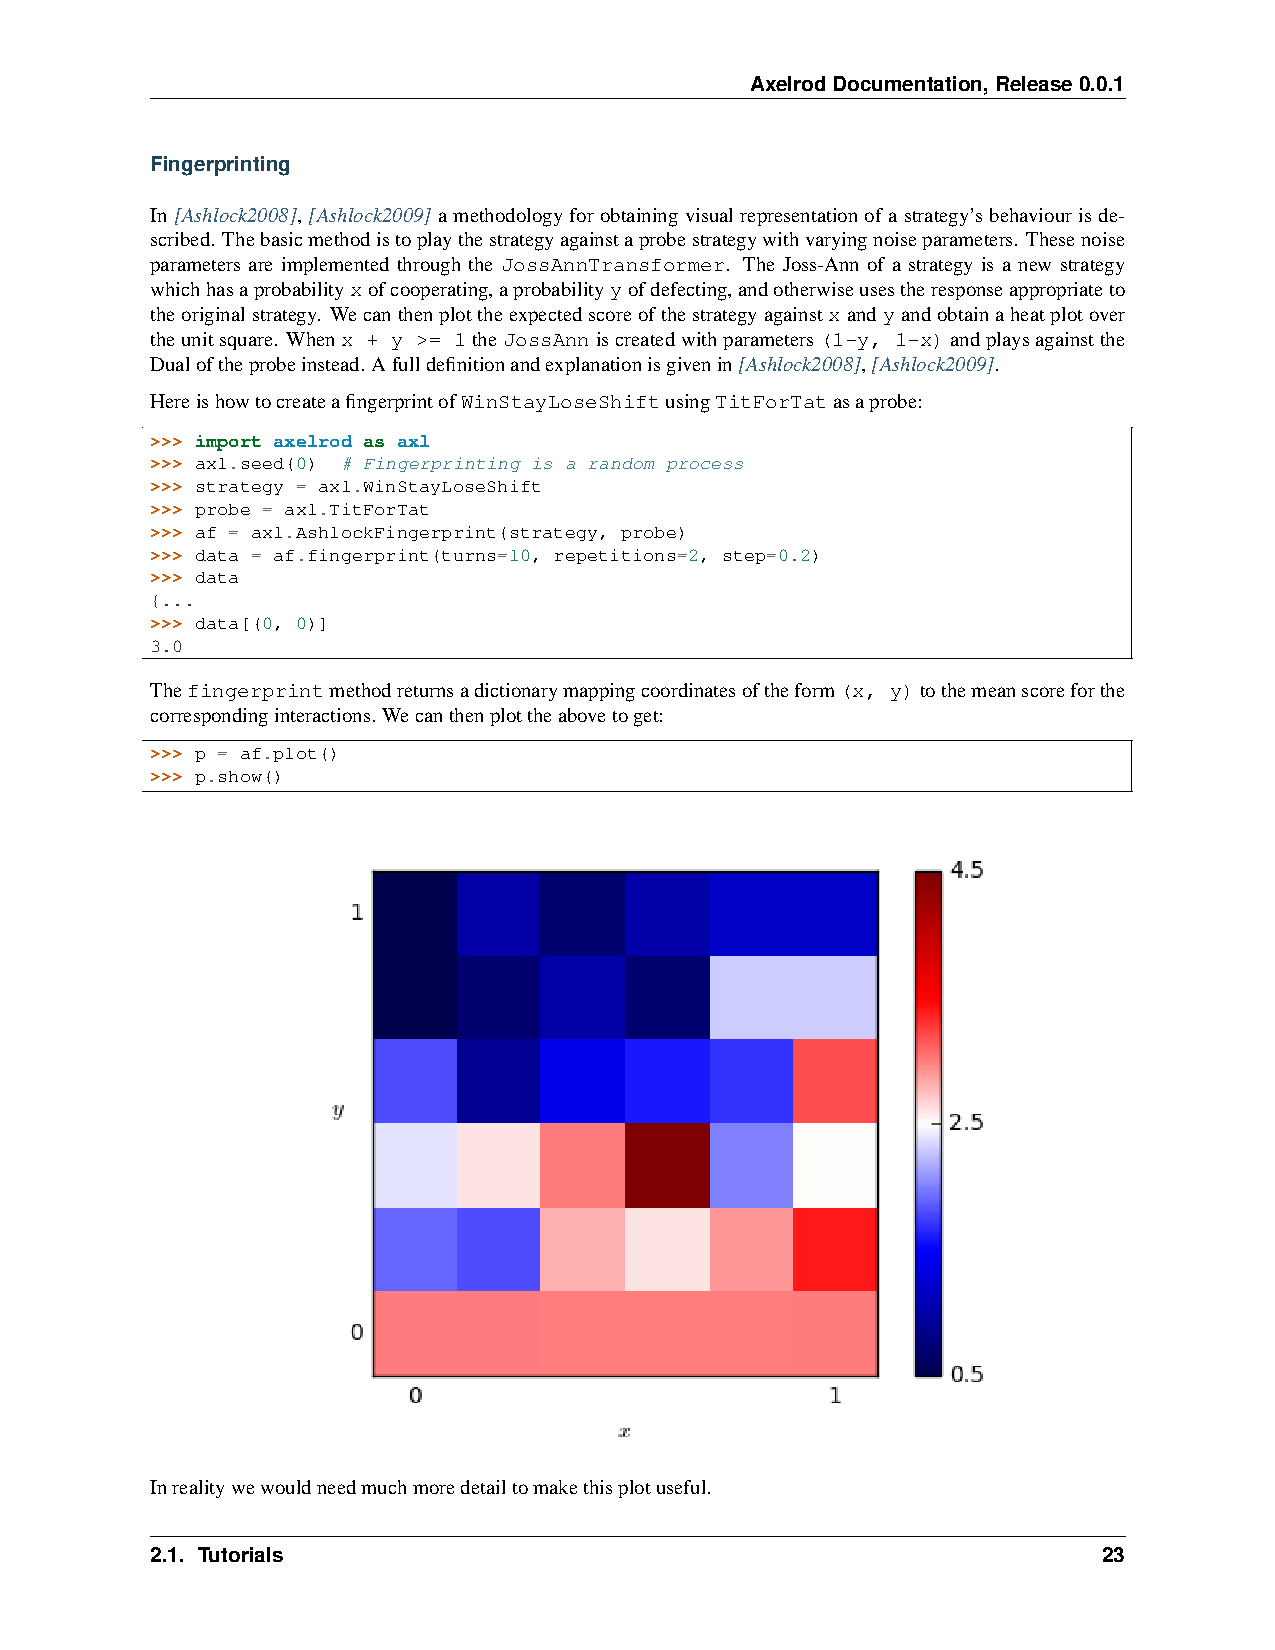
\includepdf[pages=-]{appendices/fingerprint_docs.pdf}



\section{Jupyter Notebooks}\label{app:jupyter}
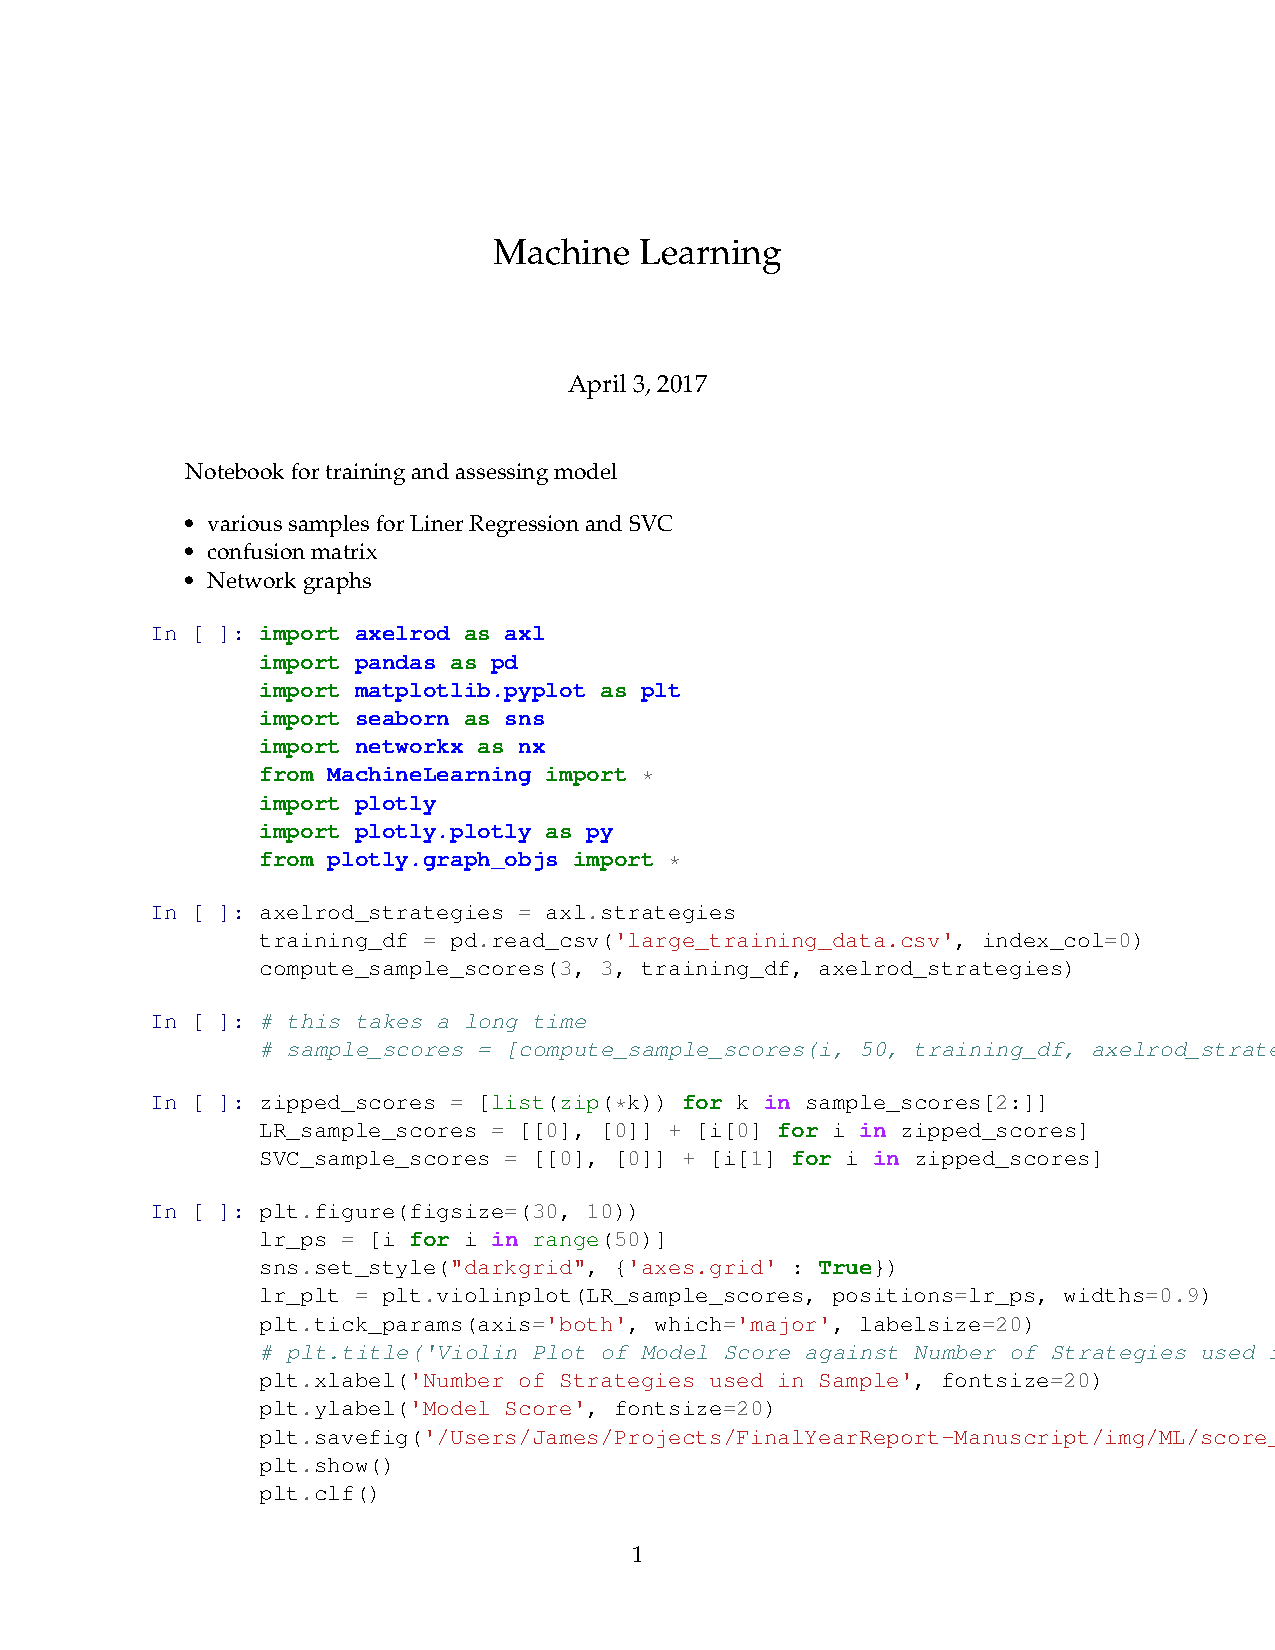
\includepdf[pages=-]{appendices/MachineLearning.pdf}
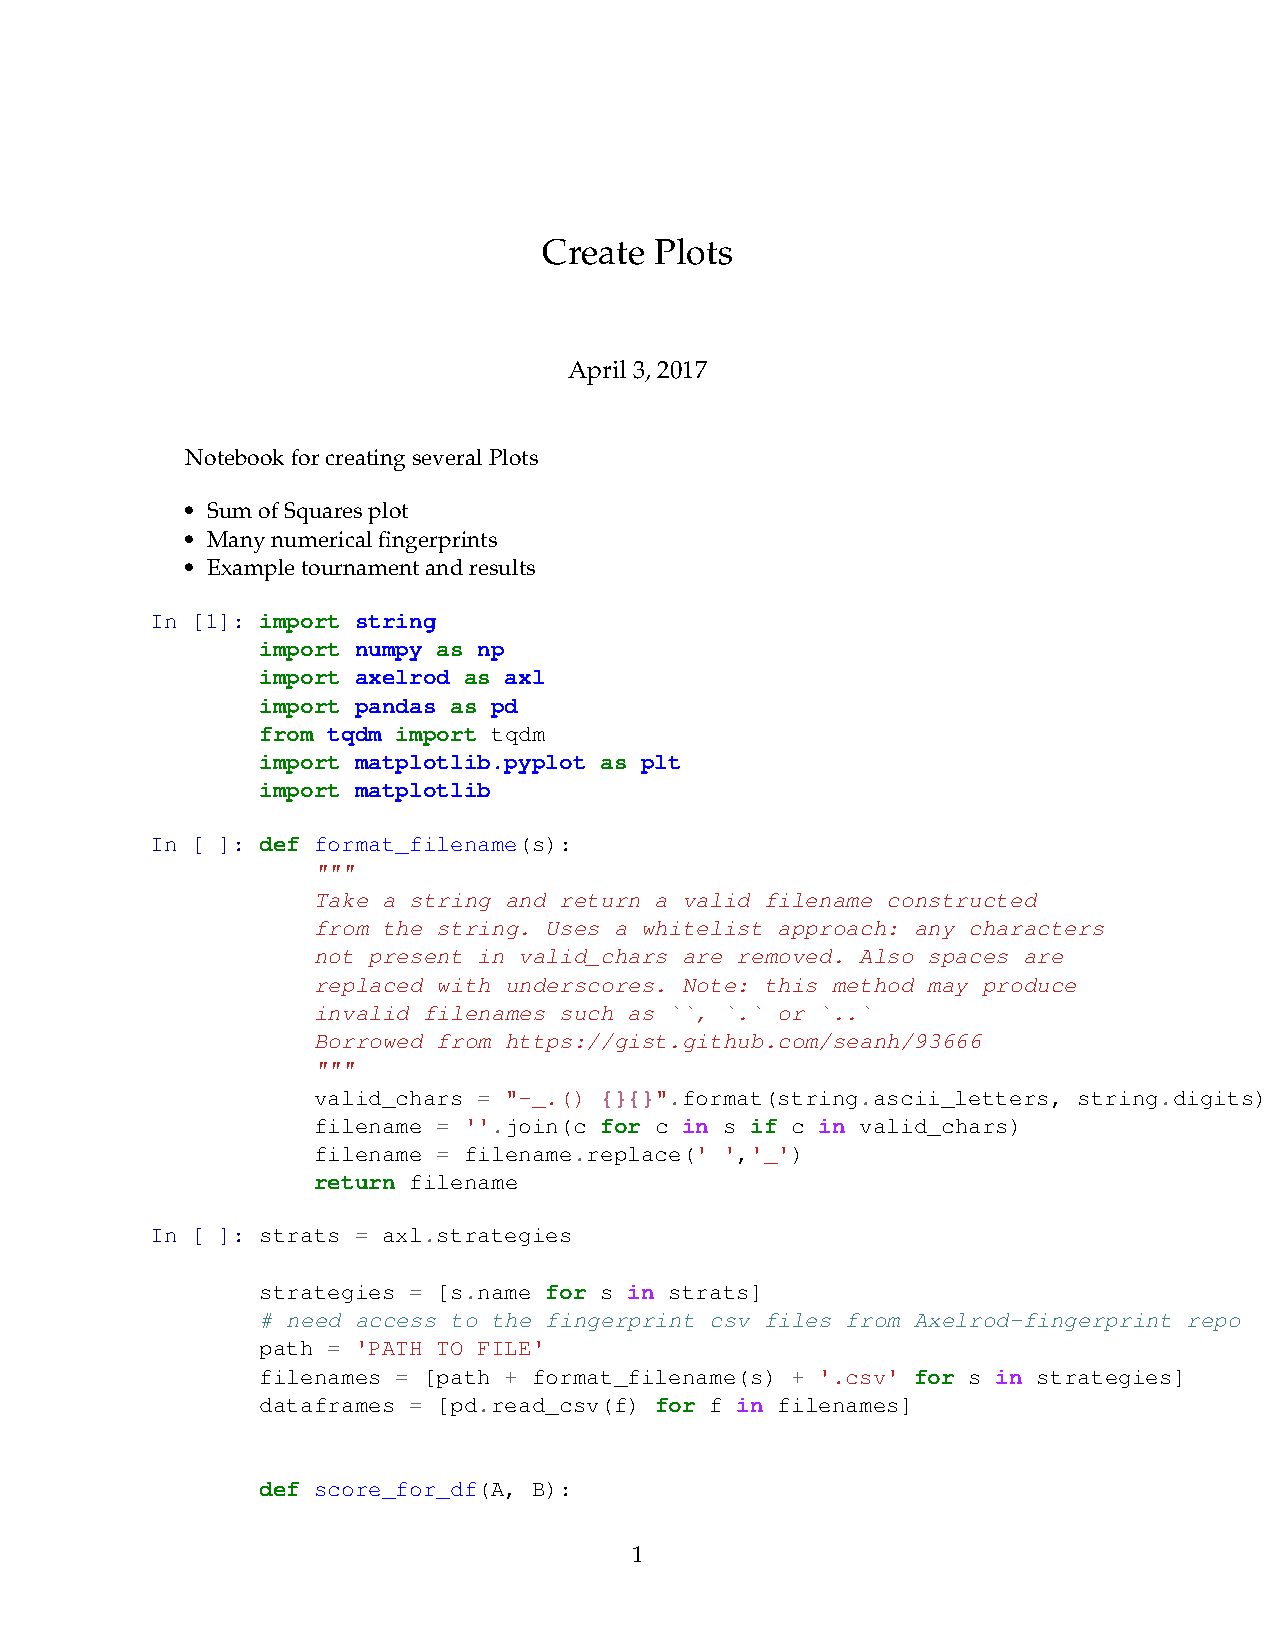
\includepdf[pages=-]{appendices/CreatePlots.pdf}
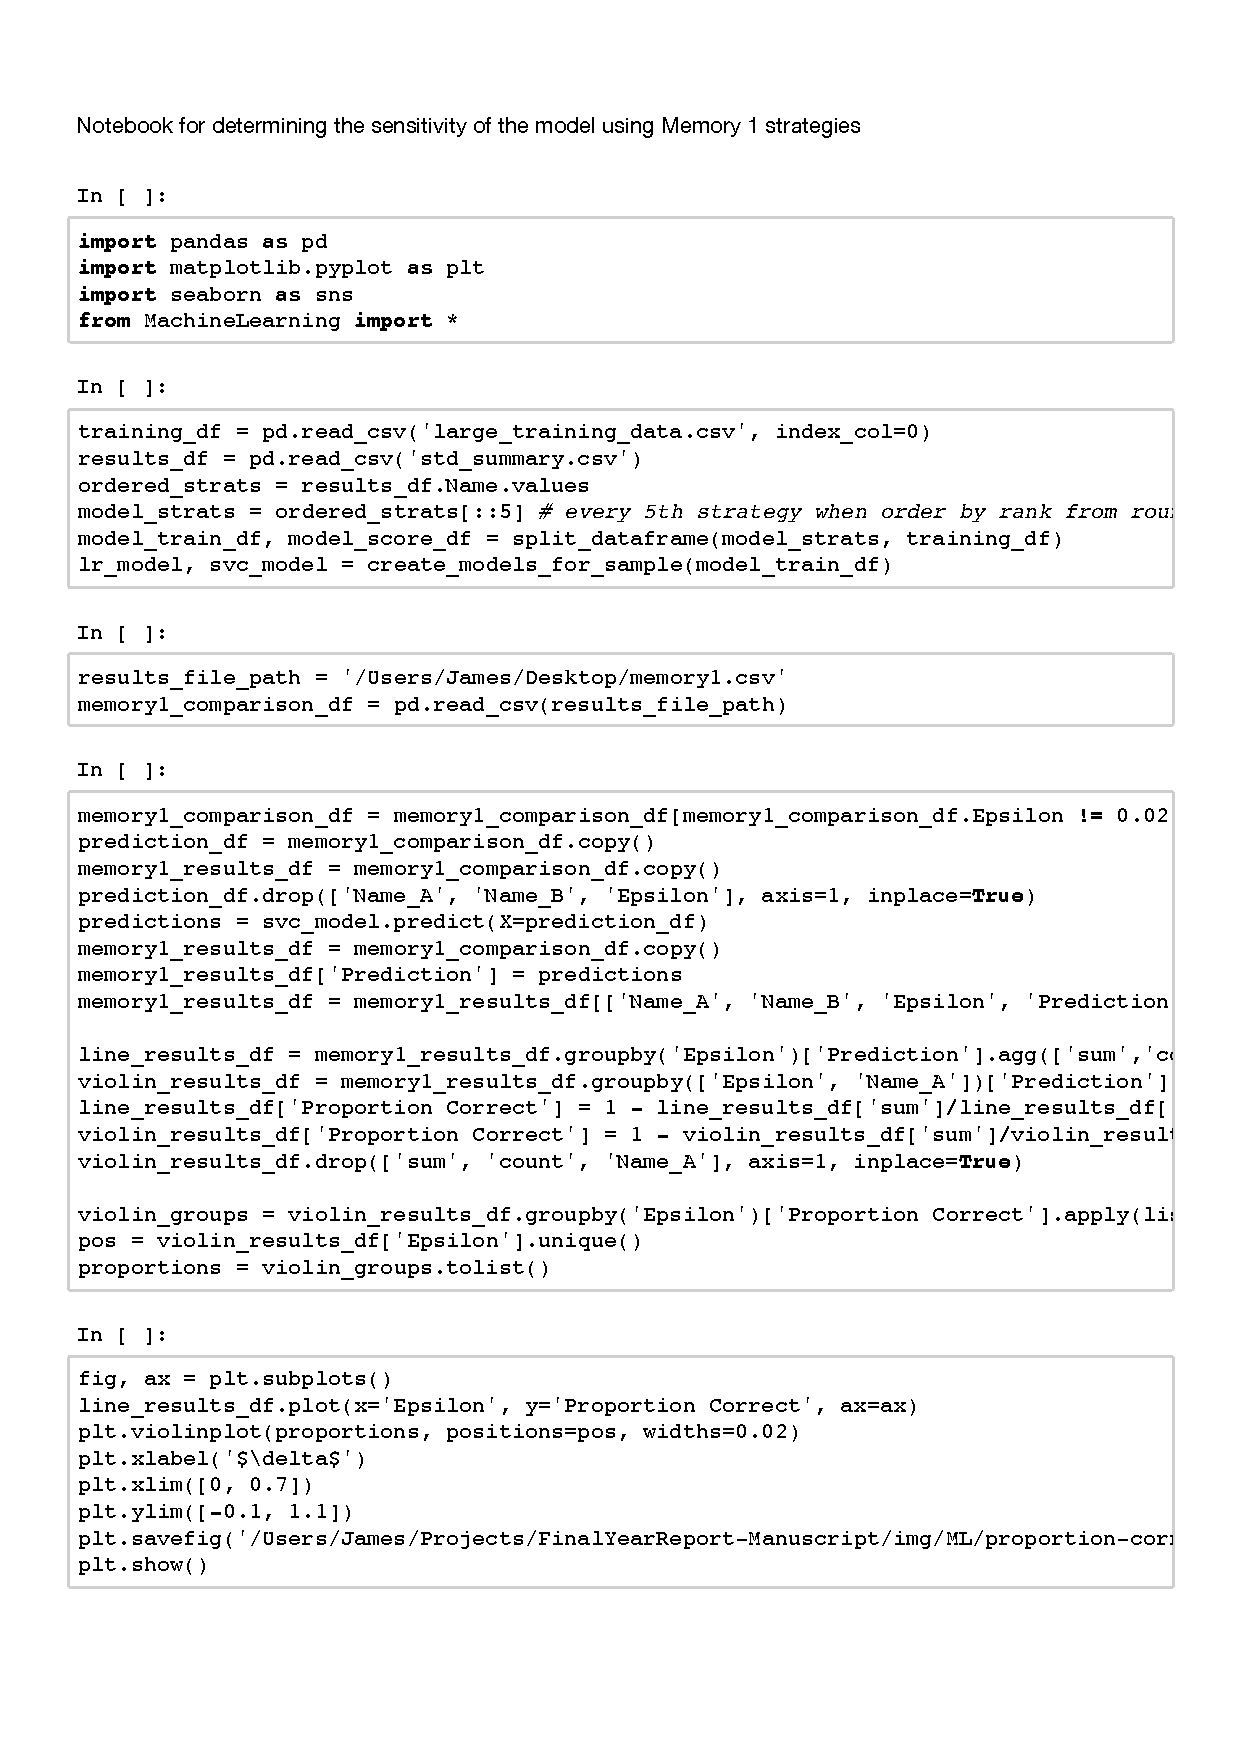
\includepdf[pages=-]{appendices/Memory1.pdf}



\section{Colour Maps}\label{app:col_maps}

\begin{figure}[htbp!]
\subfloat[Accent]{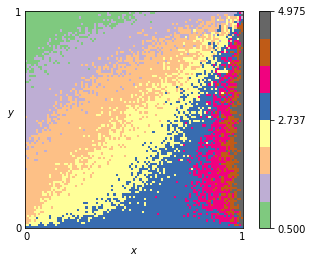
\includegraphics[width = 0.3\textwidth]{../img/ColourMaps/Accent.png}}
\subfloat[afmhot]{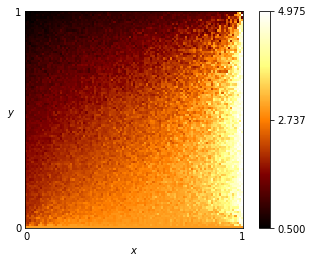
\includegraphics[width = 0.3\textwidth]{../img/ColourMaps/afmhot.png}}
\subfloat[autumn]{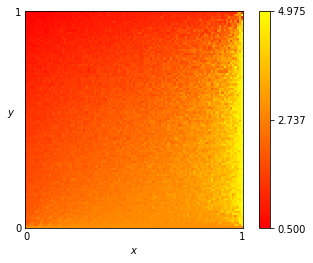
\includegraphics[width = 0.3\textwidth]{../img/ColourMaps/autumn.png}}
\phantomcaption
\end{figure}

\begin{figure}[htbp!]
\ContinuedFloat
\subfloat[binary]{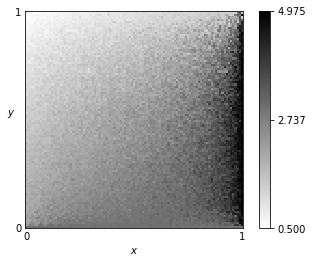
\includegraphics[width = 0.3\textwidth]{../img/ColourMaps/binary.png}}
\subfloat[Blues]{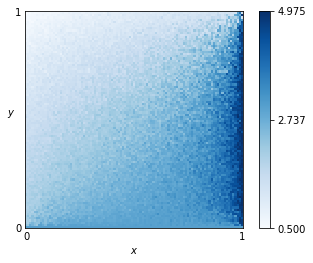
\includegraphics[width = 0.3\textwidth]{../img/ColourMaps/Blues.png}}
\subfloat[bone]{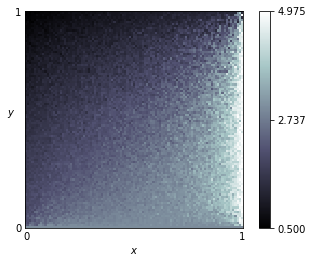
\includegraphics[width = 0.3\textwidth]{../img/ColourMaps/bone.png}}
\end{figure}

\begin{figure}[htbp!]
\ContinuedFloat
\subfloat[BrBG]{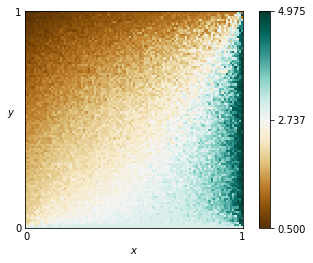
\includegraphics[width = 0.3\textwidth]{../img/ColourMaps/BrBG.png}}
\subfloat[brg]{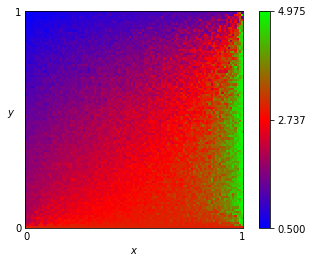
\includegraphics[width = 0.3\textwidth]{../img/ColourMaps/brg.png}}
\subfloat[BuGn]{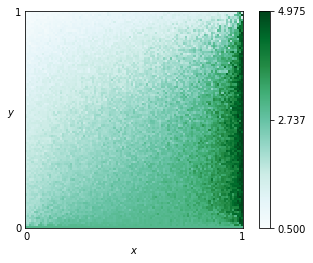
\includegraphics[width = 0.3\textwidth]{../img/ColourMaps/BuGn.png}}
\phantomcaption
\end{figure}

\begin{figure}[htbp!]
\ContinuedFloat
\subfloat[bwr]{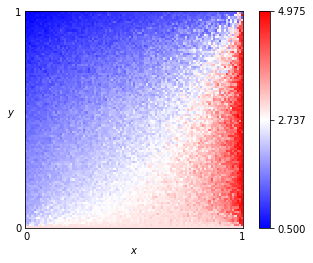
\includegraphics[width = 0.3\textwidth]{../img/ColourMaps/bwr.png}}
\subfloat[CMRmap]{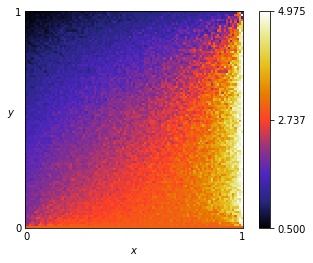
\includegraphics[width = 0.3\textwidth]{../img/ColourMaps/CMRmap.png}}
\subfloat[cool]{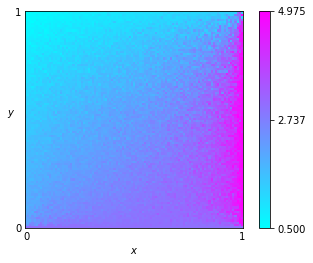
\includegraphics[width = 0.3\textwidth]{../img/ColourMaps/cool.png}}
\phantomcaption
\end{figure}

\begin{figure}[htbp!]
\ContinuedFloat
\subfloat[coolwarm]{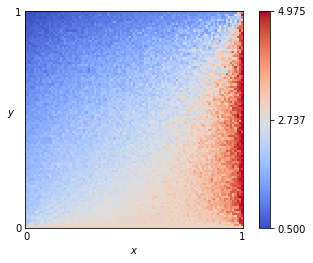
\includegraphics[width = 0.3\textwidth]{../img/ColourMaps/coolwarm.png}}
\subfloat[copper]{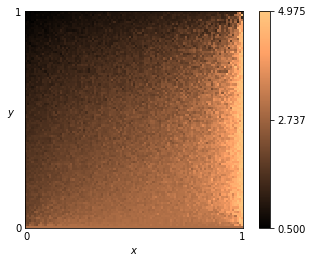
\includegraphics[width = 0.3\textwidth]{../img/ColourMaps/copper.png}}
\subfloat[cubehelix]{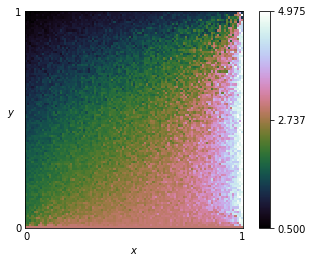
\includegraphics[width = 0.3\textwidth]{../img/ColourMaps/cubehelix.png}}
\phantomcaption
\end{figure}

\begin{figure}[htbp!]
\ContinuedFloat
\subfloat[Dark2]{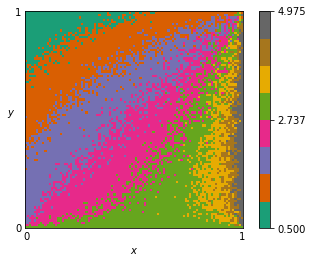
\includegraphics[width = 0.3\textwidth]{../img/ColourMaps/Dark2.png}}
\subfloat[flag]{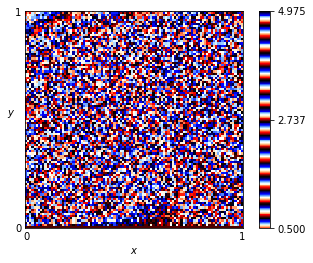
\includegraphics[width = 0.3\textwidth]{../img/ColourMaps/flag.png}}
\subfloat[gist\_earth]{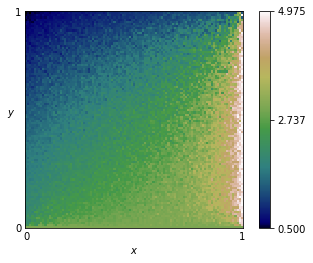
\includegraphics[width = 0.3\textwidth]{../img/ColourMaps/gist_earth.png}}
\phantomcaption
\end{figure}

\begin{figure}[htbp!]
\ContinuedFloat
\subfloat[gist\_gray]{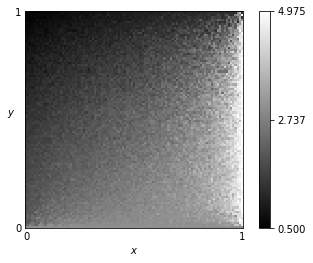
\includegraphics[width = 0.3\textwidth]{../img/ColourMaps/gist_gray.png}}
\subfloat[gist\_heat]{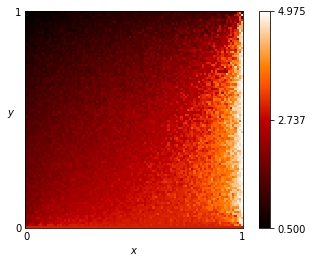
\includegraphics[width = 0.3\textwidth]{../img/ColourMaps/gist_heat.png}}
\subfloat[gist\_ncar]{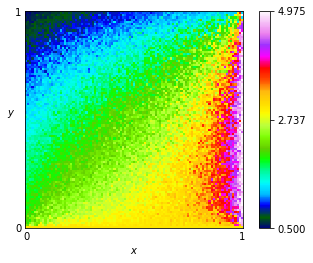
\includegraphics[width = 0.3\textwidth]{../img/ColourMaps/gist_ncar.png}}
\phantomcaption
\end{figure}

\begin{figure}[htbp!]
\ContinuedFloat
\subfloat[gist\_rainbow]{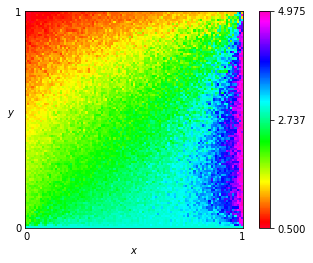
\includegraphics[width = 0.3\textwidth]{../img/ColourMaps/gist_rainbow.png}}
\subfloat[gist\_stern]{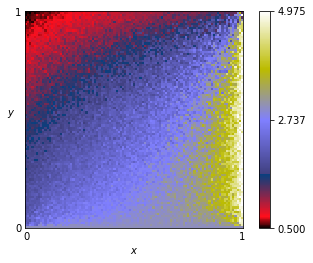
\includegraphics[width = 0.3\textwidth]{../img/ColourMaps/gist_stern.png}}
\subfloat[gist\_yarg]{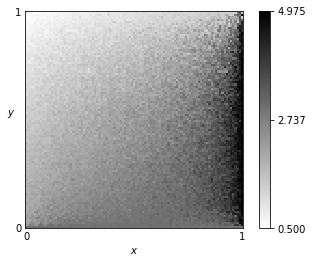
\includegraphics[width = 0.3\textwidth]{../img/ColourMaps/gist_yarg.png}}
\phantomcaption
\end{figure}

\begin{figure}[htbp!]
\ContinuedFloat
\subfloat[GnBu]{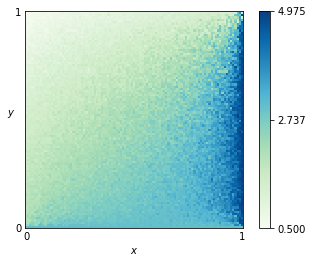
\includegraphics[width = 0.3\textwidth]{../img/ColourMaps/GnBu.png}}
\subfloat[gnuplot]{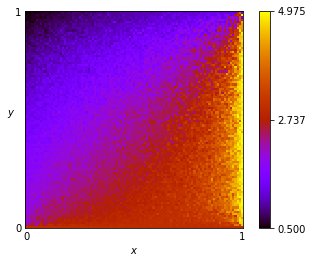
\includegraphics[width = 0.3\textwidth]{../img/ColourMaps/gnuplot.png}}
\subfloat[gnuplot2]{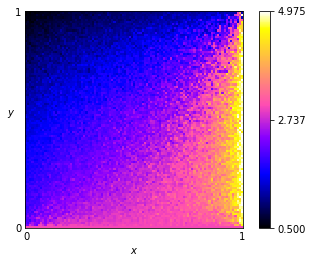
\includegraphics[width = 0.3\textwidth]{../img/ColourMaps/gnuplot2.png}}
\phantomcaption
\end{figure}

\begin{figure}[htbp!]
\ContinuedFloat
\subfloat[gray]{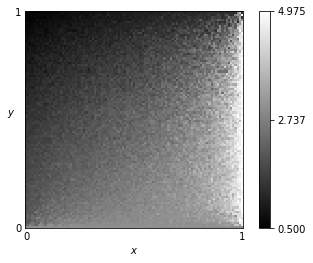
\includegraphics[width = 0.3\textwidth]{../img/ColourMaps/gray.png}}
\subfloat[Greens]{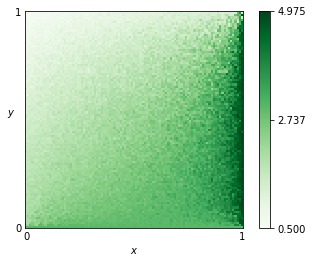
\includegraphics[width = 0.3\textwidth]{../img/ColourMaps/Greens.png}}
\subfloat[Greys]{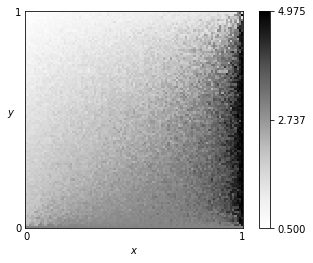
\includegraphics[width = 0.3\textwidth]{../img/ColourMaps/Greys.png}}
\phantomcaption
\end{figure}

\begin{figure}[htbp!]
\ContinuedFloat
\subfloat[hot]{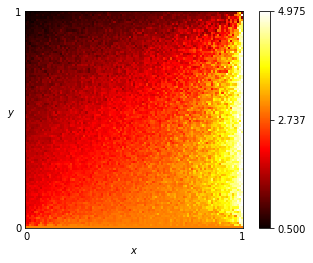
\includegraphics[width = 0.3\textwidth]{../img/ColourMaps/hot.png}}
\subfloat[hsv]{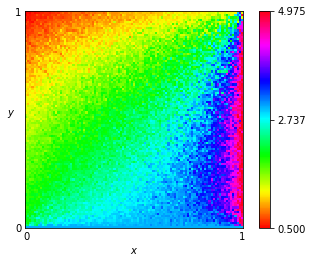
\includegraphics[width = 0.3\textwidth]{../img/ColourMaps/hsv.png}}
\subfloat[inferno]{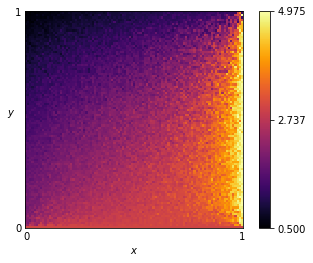
\includegraphics[width = 0.3\textwidth]{../img/ColourMaps/inferno.png}}
\phantomcaption
\end{figure}

\begin{figure}[htbp!]
\ContinuedFloat
\subfloat[jet]{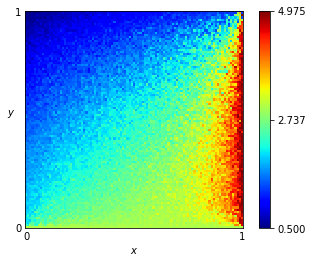
\includegraphics[width = 0.3\textwidth]{../img/ColourMaps/jet.png}}
\subfloat[magma]{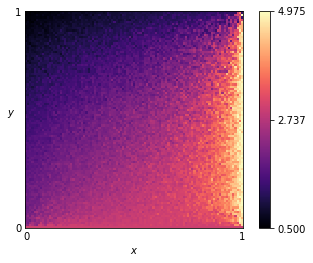
\includegraphics[width = 0.3\textwidth]{../img/ColourMaps/magma.png}}
\subfloat[nipy\_spectral]{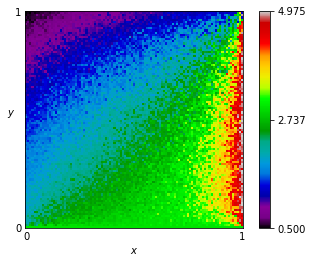
\includegraphics[width = 0.3\textwidth]{../img/ColourMaps/nipy_spectral.png}}
\phantomcaption
\end{figure}

\begin{figure}[htbp!]
\ContinuedFloat
\subfloat[ocean]{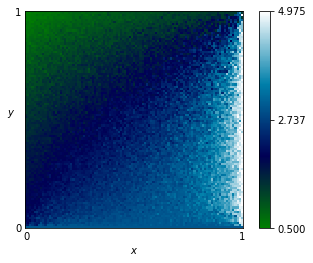
\includegraphics[width = 0.3\textwidth]{../img/ColourMaps/ocean.png}}
\subfloat[Oranges]{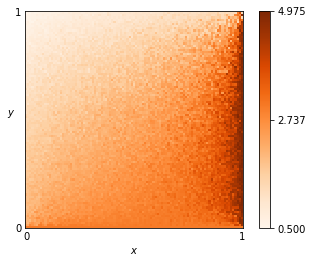
\includegraphics[width = 0.3\textwidth]{../img/ColourMaps/Oranges.png}}
\subfloat[OrRd]{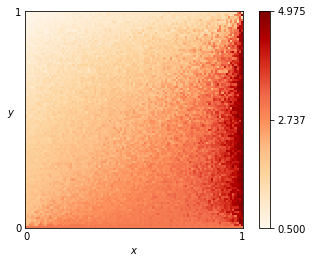
\includegraphics[width = 0.3\textwidth]{../img/ColourMaps/OrRd.png}}
\phantomcaption
\end{figure}

\begin{figure}[htbp!]
\ContinuedFloat
\subfloat[Paired]{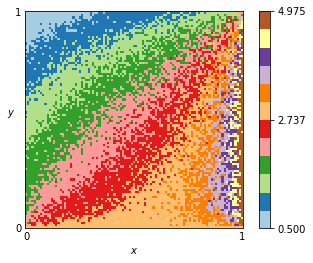
\includegraphics[width = 0.3\textwidth]{../img/ColourMaps/Paired.png}}
\subfloat[Pastel1]{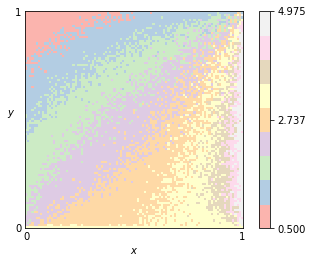
\includegraphics[width = 0.3\textwidth]{../img/ColourMaps/Pastel1.png}}
\subfloat[Pastel2]{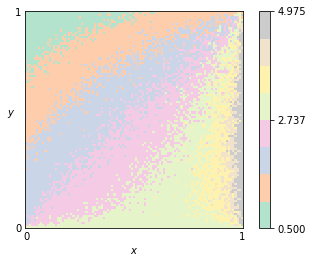
\includegraphics[width = 0.3\textwidth]{../img/ColourMaps/Pastel2.png}}
\phantomcaption
\end{figure}

\begin{figure}[htbp!]
\ContinuedFloat
\subfloat[pink]{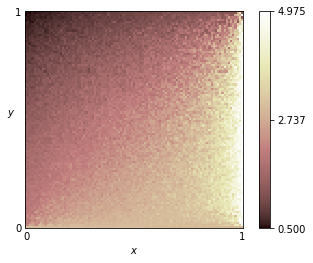
\includegraphics[width = 0.3\textwidth]{../img/ColourMaps/pink.png}}
\subfloat[PiYG]{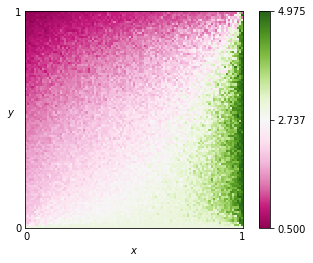
\includegraphics[width = 0.3\textwidth]{../img/ColourMaps/PiYG.png}}
\subfloat[plasma]{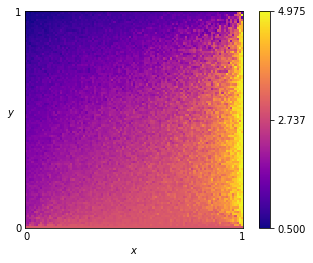
\includegraphics[width = 0.3\textwidth]{../img/ColourMaps/plasma.png}}
\phantomcaption
\end{figure}

\begin{figure}[htbp!]
\ContinuedFloat
\subfloat[PRGn]{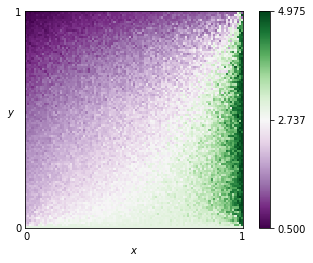
\includegraphics[width = 0.3\textwidth]{../img/ColourMaps/PRGn.png}}
\subfloat[prism]{\includegraphics[width = 0.3\textwidth]{../img/ColourMaps/prism.png}}
\subfloat[PuBu]{\includegraphics[width = 0.3\textwidth]{../img/ColourMaps/PuBu.png}}
\phantomcaption
\end{figure}

\begin{figure}[htbp!]
\ContinuedFloat
\subfloat[PuBuGn]{\includegraphics[width = 0.3\textwidth]{../img/ColourMaps/PuBuGn.png}}
\subfloat[PuOr]{\includegraphics[width = 0.3\textwidth]{../img/ColourMaps/PuOr.png}}
\subfloat[PuRd]{\includegraphics[width = 0.3\textwidth]{../img/ColourMaps/PuRd.png}}
\phantomcaption
\end{figure}

\begin{figure}[htbp!]
\ContinuedFloat
\subfloat[Purples]{\includegraphics[width = 0.3\textwidth]{../img/ColourMaps/Purples.png}}
\subfloat[rainbow]{\includegraphics[width = 0.3\textwidth]{../img/ColourMaps/rainbow.png}}
\subfloat[RdBu]{\includegraphics[width = 0.3\textwidth]{../img/ColourMaps/RdBu.png}}
\phantomcaption
\end{figure}

\begin{figure}[htbp!]
\ContinuedFloat
\subfloat[RdGy]{\includegraphics[width = 0.3\textwidth]{../img/ColourMaps/RdGy.png}}
\subfloat[RdPu]{\includegraphics[width = 0.3\textwidth]{../img/ColourMaps/RdPu.png}}
\subfloat[RdYlBu]{\includegraphics[width = 0.3\textwidth]{../img/ColourMaps/RdYlBu.png}}
\phantomcaption
\end{figure}

\begin{figure}[htbp!]
\ContinuedFloat
\subfloat[RdYlGn]{\includegraphics[width = 0.3\textwidth]{../img/ColourMaps/RdYlGn.png}}
\subfloat[Reds]{\includegraphics[width = 0.3\textwidth]{../img/ColourMaps/Reds.png}}
\subfloat[seismic]{\includegraphics[width = 0.3\textwidth]{../img/ColourMaps/seismic.png}}
\phantomcaption
\end{figure}

\begin{figure}[htbp!]
\ContinuedFloat
\subfloat[Set1]{\includegraphics[width = 0.3\textwidth]{../img/ColourMaps/Set1.png}}
\subfloat[Set2]{\includegraphics[width = 0.3\textwidth]{../img/ColourMaps/Set2.png}}
\subfloat[Set3]{\includegraphics[width = 0.3\textwidth]{../img/ColourMaps/Set3.png}}
\phantomcaption
\end{figure}

\begin{figure}[htbp!]
\ContinuedFloat
\subfloat[Spectral]{\includegraphics[width = 0.3\textwidth]{../img/ColourMaps/Spectral.png}}
\subfloat[spring]{\includegraphics[width = 0.3\textwidth]{../img/ColourMaps/spring.png}}
\subfloat[summer]{\includegraphics[width = 0.3\textwidth]{../img/ColourMaps/summer.png}}
\phantomcaption
\end{figure}

\begin{figure}[htbp!]
\ContinuedFloat
\subfloat[terrain]{\includegraphics[width = 0.3\textwidth]{../img/ColourMaps/Vega10.png}}
\subfloat[Vega10]{\includegraphics[width = 0.3\textwidth]{../img/ColourMaps/OrRd.png}}
\subfloat[Vega20]{\includegraphics[width = 0.3\textwidth]{../img/ColourMaps/Vega20.png}}
\phantomcaption
\end{figure}

\begin{figure}[htbp!]
\ContinuedFloat
\subfloat[Vega20b]{\includegraphics[width = 0.3\textwidth]{../img/ColourMaps/Vega20b.png}}
\subfloat[Vega20c]{\includegraphics[width = 0.3\textwidth]{../img/ColourMaps/Vega20c.png}}
\subfloat[viridis]{\includegraphics[width = 0.3\textwidth]{../img/ColourMaps/viridis.png}}
\phantomcaption
\end{figure}

\begin{figure}[htbp!]
\ContinuedFloat
\subfloat[winter]{\includegraphics[width = 0.3\textwidth]{../img/ColourMaps/winter.png}}
\subfloat[Wistia]{\includegraphics[width = 0.3\textwidth]{../img/ColourMaps/Wistia.png}}
\subfloat[YlGn]{\includegraphics[width = 0.3\textwidth]{../img/ColourMaps/YlGn.png}}
\phantomcaption
\end{figure}

\begin{figure}[htbp!]
\ContinuedFloat
\subfloat[YlGnBu]{\includegraphics[width = 0.3\textwidth]{../img/ColourMaps/YlGnBu.png}}
\subfloat[YlOrBr]{\includegraphics[width = 0.3\textwidth]{../img/ColourMaps/YlOrBr.png}}
\subfloat[YlOrRd]{\includegraphics[width = 0.3\textwidth]{../img/ColourMaps/YlOrRd.png}}

\caption{All possible colour maps from Matplotlib}
\label{fig:col_maps}
\end{figure}
